\documentclass[12pt,a4paper,oneside]{article}
\usepackage{amsmath}
\usepackage{amssymb}
\usepackage{graphicx}
\usepackage{indentfirst}
\usepackage{listings}
\usepackage{hyperref}
\usepackage{wrapfig}
\usepackage{caption}
\usepackage{subcaption}
\usepackage{float}
\usepackage{amsmath}
\usepackage{setspace}
\usepackage{standalone}

\setlength{\voffset}{-28.4mm}
\setlength{\hoffset}{-1in}
\setlength{\topmargin}{20mm}
\setlength{\oddsidemargin}{25mm}
\setlength{\evensidemargin}{25mm}
\setlength{\textwidth}{160mm}

\setlength{\parindent}{0pt}

\setlength{\textheight}{235mm}
\setlength{\footskip}{20mm}
\setlength{\headsep}{50pt}
\setlength{\headheight}{0pt}

\begin{document}
\pagestyle{empty}
%%%% Title page
\begin{titlepage}
\begin{center}

\includegraphics[scale=0.4]{ebi_logo.png} \thinspace \thinspace \thinspace

\includegraphics[scale=0.6]{uni_cam_logo.jpg}\\[5mm]
\vspace*{20mm}
\sf
\normalsize

\bigskip
{\Huge

  \textbf{Reconstructing mutational patterns in model organisms and primary cancer samples}
}
\bigskip

\vspace*{30mm}

\normalsize
{\Large
Nadezda Volkova
}
\end{center}

\end{titlepage}

\tableofcontents
\newpage{}


\begin{document}
\pagestyle{empty}

\chapter{Introduction}

Genome stability maintenance plays the key role in cell’s ability to propagate. Spontaneous 
changes and mutagenic damage in the genome may cause wide range of diseases including cancer. 
These alterations can be an effect of combination of environmental factors damaging DNA and 
deficiencies in DNA repair and replication leading to characteristic mutational spectra.

Various mutational process attack the genome due to endogenous or exogenous factors, and 
many of them are believed to leave a unique pattern of mutations in the genome. Given the 
explosion in the amount of publicly available cancer sequencing data, it was tempting to 
aggregate it together and apply machine learning methods to extract the signatures of 
underlying mutagenic processes. Hence, mutational signatures (\cite{Alexandrov2013-md}, 
\cite{Alexandrov2015-clock}, \cite{Nik-Zainal2012-eg}) became a very useful tool of cancer 
investigation in the last years. However, most of the signatures identified so far represent 
complex conglomerates of the action of different mutational processes, deciphering which will 
be essential for understanding the causes of the disease and the most efficient treatment 
options. For some of the signatures, significant associations with various mutational 
processes were identified, although the precise causation is still unclear (\cite{Alexandrov2013-md},
\cite{Alexandrov2015-clock}, \cite{Helleday2014-kw}). For others, no links with the underlying 
mutational processes were found so far. 

The mutational profiles observed in sequencing studies represent the result of interaction 
between damaging and repairing factors, and the ability to disentangle the interactions 
between them which are shaping mutational history of a tumor gives more insight into the 
origins of a particular tumor and may suggest prospective targets for treatment 
(\cite{Alexandrov2013-zu}, \cite{Alexandrov2015-gastric}, \cite{Hollstein2017-ag}, \cite{Poon2014-review}). 
Dissecting the individual contributions of each of DNA repair deficiencies and external 
exposures represents a highly complex task due to  redundancy in DNA repair pathways, 
interaction effects, sequencing artifacts, and high inter- and intra-personal variance 
among patients. Hence the investigation of mutational patterns in a controlled environment 
of a model organism can give a better understanding of underlying biology and shed light 
on the precise contribution of the factors involved (\cite{Meier2014-aa}, \cite{Segovia2015-cr}).

DNA repair mechanisms represent the key component of genome stability maintenance. 
Repair ability deficiencies provide space for major alterations of the genome, both 
by the aggregation of spontaneous mutations and the lack of mutagen resistance. 
There are several major classes of DNA repair pathways: direct reversal, single-strand 
damage repair (such as base excision repair, nucleotide excision repair and mismatch 
repair systems), double-strand break repair (which includes homologous recombination, 
microhomology-mediated end joining and non-homologous end-joining), translesion synthesis, 
and also DNA damage signaling pathways and associated cell cycle control mechanisms 
(\cite{Alberts2007-qn}). Dissecting the individual contribution of each of them represents 
a highly complex task, since many DNA repair components have functions associated with 
different repair pathways, and in some cases these mechanisms may be interchangeable. 
Nevertheless it is possible to investigate the contributions of the most essential 
genetic components and their interplay with each other and with various cytotoxins 
to imitate the processes happening in cancer (\cite{Helleday2014-kw}, \cite{Wu2016-qp}).

The central conceptual parameter of cancer development are the driver genes that 
cause the most important events in individual cancer evolution (\cite{Stratton2009-kh}). 
The set of driver mutations is usually small, but most of them happen in the genes 
essential for cell growth or damage-caused apoptosis (such as tumor suppressor gene 
P53 (\cite{Rivlin2011-cz}) or oncogene KRAS (\cite{Wang2015-ki}) and lead to bursts of mutations directed 
by the effectiveness of particular DNA repair mechanisms. Knowing the individual and 
interaction effects of key elements of genome stability maintenance and environmental 
exposures will provide means to trace back the causes of the disease and predict the 
outcomes of chemo- or radiotherapy in every individual case (\cite{Poon2014-review}).

%%%%%%%%%%%%%%%%%%%%%%%%%%%%%%%%%%%%%%%%%%%%%%%%%

\begin{document}
\pagestyle{empty}
\section{Mutagenesis}

%%%%%%%%%%%%%%%%%%%%%%%%%%%%%%%%%%%%%%%%%%%%%%%%%%%%%%%%%%%%%

\subsection{History of mutagenesis research}

\todo[inline]{collect some reviews on mutagenesis in different model organisms}

%%%%%%%%%%%%%%%%%%%%%%%%%%%%%%%%%%%%%%%%%%%%%%%%%%%%%%%%%%%%%

\subsection{DNA repair and DNA damage}

\subsubsection{Types of DNA damage}

\subsubsection*{Environmental and intrinsic damage sources}

\subsubsection{DNA repair pathways and related diseases}

\subsubsection*{Direct repair}

\subsubsection*{Mismatch repair}

Fidelity of replication is maintained via multiple mechanisms: replicative polymerases 
Pol $\epsilon$ and Pol $\delta$ possess high selectivity against mismatches as well as a 
3'-exonuclease activity, and also backed up by a postreplicative repair pathway - DNA mismatch repair.
It is initiated by the recognition of replication errors left by the replicative polymerase, which 
has an error rate of about $10^{-5}$ to $10^{-4}$ (\cite{kunkel2000dna}) depending on the nucleotide,
local chromosomal properties and DNA polymerase.

The recognition of mismatches is performed by MutS protein complexes first found in bacteria *REF*.
In eukatyotes (???), there are two complexes: MutS$\alpha$, which consists of MSH2 and MSH6 proteins, 
and MutS$\beta$ cosisting of MSH2 and MSH3. Due to different mismatch binding sites, they have 
different substrate specificity: MutS-$\alpha$ preferentially detects base-base mismatches and short 1-2bp indels,
and MutS-$\beta$ handles larger indels up to 15 bp (\cite{Drummond1995-gc}, \cite{Habraken1996-vc}, 
\cite{Genschel1998-by}). MutS proteins form a clamp sliding along the genome, which is activated upon an
encounter with a mismatch and loads the other repair complex MutL to license excision.

%%%%%%% to be rewritten later %%%%%%%%%%%

Binding of MutS proteins to the DNA lesion facilitates subsequent recruitment of 
the MutL complex. MutL enhances mismatch recognition and 
promotes a conformational change in MutS through ATP hydrolysis to allow for the sliding of the MutL/MutS 
complex away from mismatched DNA (Allen, Gradia). DNA repair is initiated in most systems by a single-stranded 
nick generated by MutL (MutH in \textit{E. coli}) on the nascent DNA strand at some distance to the lesion 
(Kadyrov, Kadyrov2). Exonucleolytic activities in part conferred by Exo1 contribute to the removal of the DNA 
stretch containing the mismatch followed by gap filling via lagging strand DNA synthesis (Szankasi, Longley, 
Tishkoff, Genschel, Genschel and Modrich 2003, Constantin et al. 2005, Goellner et al. 2015). The most 
prominent MutL activity in human cells is provided by the MutL-$\alpha$ heterodimer, MLH1/PMS2 (Prolla et al. 1998; 
Cannavo et al. 2005). However, human MLH1 is also found in heterodimers with PMS1 and MLH3, called 
MutL-$\beta$ and MutL-$\gamma$. Of these two only MutL-$\gamma$ is thought to have a minor role in MMR 
(Cannavo et al. 2005). In \textit{C. elegans}, MLH-1 and PMS-2 are the only MutL homologs encoded in the genome.


A large number of studies have analyzed mutations arising in DNA mismatch repair deficient cells at specific 
genomic loci or in reporter constructs. Analysis of microsatellite loci in \textit{mlh1} deficient 
colorectal cancer cell lines suggested rates of repeat expansions or contractions between 
$8.4 \cdot 10^{-3}$ to $3.8 \cdot 10^{-2}$ per locus and generation 
(Bhattacharyya et al. 1994; Hanford et al. 1998). Estimates using \textit{S. cerevisiae} 
revealed a 100- to 700-fold increase in DNA repeat tract instability in \textit{pms2}, 
\textit{mlh1} and \textit{msh2} mutants (Strand et al. 1993) and a ~5-fold increase in 
base substitution rates (Yang et al. 1999). \textit{C. elegans} assays using reporter 
systems or selected, PCR-amplified regions revealed a more than 30-fold increased 
frequency of single base substitutions in msh-6, a 500-fold increase in mutations 
in A/T homopolymer runs and a 100-fold increase in mutations in dinucleotide repeats 
(Degtyareva et al. 2002; Tijsterman et al. 2002; Denver et al. 2005), akin to the 
frequencies observed in yeast and mammalian cells (Strand et al. 1993; Hanford et al. 1998). 
Recently, whole genome sequencing approaches using diploid S. cerevisiae started to provide 
a genome-wide view of MMR deficiency. \textit{S. cerevisiae} lines carrying an \textit{msh2} 
deletion alone or in conjunction with point mutations in one of the three replicative 
polymerases, Pol $\alpha$/primase, Pol-$\delta$, and Pol-$\epsilon$, were propagated over 
multiple generations to determine the individual contribution of replicative polymerases 
and MMR to replication fidelity (Lang et al. 2013; Lujan et al. 2014; Lujan et al. 2015). 
These analyses observed an average base substitution rate of 1.6 x 10-8 per base pair per 
generation in msh2 mutants and an increased rate in mutants in which \textit{msh2} and one 
of the replicative polymerases was mutated (Lujan et al. 2014; Lujan et al. 2015). 
A synergistic increase in mutagenesis was also recently observed in childhood tumors in 
which MMR deficiency and mutations in replicative polymerase $\epsilon$ and $\delta$ 
needed for leading and lagging strand DNA synthesis occurred \cite{Shlien}. 

\subsubsection*{Nucleotide excision repair}

\subsubsection*{Base excision repair}

\subsubsection*{Crosslink repair}

\subsubsection*{Single strand break repair}

\subsubsection*{Double strand break repair}

\subsubsection*{Translesion synthesis}

\subsubsection*{DNA damage response regulation}

%%%%%%%%%%%%%%%%%%%%%%%%%%%%%%%%%%%%%%%%%%%%%%%%%%%%%%%%%%%%%

\subsection{Methods for detection of DNA damage and DNA repair}

\end{document}

%%%%%%%%%%%%%%%%%%%%%%%%%%%%%%%%%%%%%%%%%%%%%%%%%


\begin{document}
\pagestyle{empty}

%%%%%%%%%%%%%%%%%%%%%%%%%%%%%%%%%%%%%%%%%%%%%%%%%%%%%%%%%%%%%

\section{Mutational signatures}

%%%%%%%%%%%%%%%%%%%%%%%%%%%%%%%%%%%%%%%%%%%%%%%%%%%%%%%%%%%%%

\subsection{Somatic mutations in cancer}

\subsection*{Mutagen exposure, DNA repair deficiencies and cancer risk}

\subsection*{Driver and passenger mutations}



%%%%%%%%%%%%%%%%%%%%%%%%%%%%%%%%%%%%%%%%%%%%%%%%%%%%%%%%%%%%%


\subsection{Concept of mutational signatures}

\subsection*{Individual factor analysis in human cancer }

Signatures inferred from model organisms are essential for the understanding of mutagenesis mechanisms. 
Apart from the significance for basic research, it would be of great importance to  translate these 
effects into human data as it would allow to study the causes of the diseases caused by acquired 
changes in DNA, and first of all of cancer.

The main difficulty consists in constructing an adequate transformation of the signatures 
obtained using worm data in order to apply them to other organism. We are planning to 
normalize the signatures as much as possible using functional and chemical features 
available for \textit{C. elegans} and further validate them by the use of yeast and 
human iPS cell lines data from COMSIG.

Using these translated signatures, we plan to perform single mutagenic factor based 
analysis of the primary cancer samples from TCGA. There are two strategies we are 
going to apply in order to establish the links between mutational factor signatures 
and tumor DNA alteration spectra:

\begin{itemize}
\item Investigate the samples with known exposures and DNA repair deficiencies in 
order to estimate individual contributions of different factors into the overall 
mutational landscape of each cancer sample. 
\item Try to identify the patterns caused by individual factors in primary cancer 
samples and link them back to the cancer types the samples are coming from.
\end{itemize}

After proving applicability of the individual factor signatures to human data,
we will be able to start a deeper investigation of mutational signatures in 
cancers and their underlying mechanisms.


\subsection*{Cancer genome decomposition}

According to the current state of the Catalogue Of Somatic Mutations In Cancer (COSMIC) project
(\cite{Forbes2015-gf}), there are 30 base substitution signatures identified so far (several indel 
and genomic rearrangement signatures identified recently (e.g. \cite{Alexandrov2015-clock}, \cite{Nik-Zainal2012-eg}) are 
not included in the catalogue yet). It is important to notice that these signatures may be 
not unique: they were extracted from a large dataset of cancer genomes as one possible basis 
of the latent variable space, and their linear combination may represent more meaningful 
signatures (e.g., as was proven for signatures 1A, 1B and 5 in \cite{Alexandrov2015-clock}), expecially as 
soon as more data is added to the pool, increasing the statistical power of blind source 
separation methods such as NMF (\cite{Alexandrov2013-zu}).

In human cancer samples 30 mutational signatures (referred to as COSMIC signatures 
from here on) have been uncovered by mathematical modeling across a large number of cancer genomes representing more
than 30 tumor types (http://cancer.sanger.ac.uk/cosmic/signatures) (Alexandrov 2013a; 
Alexandrov 2013b). These signatures are largely define by the relative frequency of the six possible 
base substitutions (C>A, C>G, C>T, T>A, T>C, T>G), occurring in a sequence context defined by their
adjacent 5’ and 3’ base. Of these, COSMIC signatures 6, 15, 20, 21 and 26, have been associated 
with MMR deficiency with several MMR signatures being present in the same tumor sample.

Based on large cohort studies, several significant associations were identified for 
17 base substitution signatures with both genetic and environmental factors (\cite{Alexandrov2013-md},\cite{Alexandrov2015-clock},\cite{Roberts2014-nl}):

\begin{itemize}
\itemsep0em
\item Genetic factors:
  \begin{itemize}
  \itemsep0em
  \item Signatures 1 and 5 are strongly correlated with age and may therefore represent aging related mutational processes (\cite{Alexandrov2015-clock});
  \item Signatures 2 and 13 were associated with the activity of APOBEC family related pathways;
  \item Signature 3 - with defective homologous recombination;
  \item Signatures 6, 15, 20 and 26 - with DNA mismatch repair deficiency (\cite{Supek2015-pr});
  \item Signatures 9 and 10 are associated with polymerases failures;
  \end{itemize}
\item Mutagen exposures:
  \begin{itemize}
  \itemsep0em
  \item Signature 24 has a proposed link to aflatoxin exposure;
  \item Signatures 4 and 29 have been attributed to tobacco mutagenesis;
  \item Signature 7 is potentially associated with UV;
  \item Signature 11 - with the action of an alkylating agent temozolomide (\cite{Poon2014-review});
  \item Signature 22 was only found in the samples with aristolochic acid exposure (\cite{Poon2015-AA});
  \end{itemize}
\end{itemize}

In order to further explain the mutational background of cancer, we propose to perform the following steps:

\begin{enumerate}
\item Assess cancer signature purity by direct comparison of individual factor signatures with the respective cancer-type dependent signature combinations.
\item Search for the further associations between the signatures and individual genetic and mutagenic components from the catalogue, measure the contribution of interaction factors.
\item Potentially recombine the signatures into new linear combinations which would be explicitly linked to a particular mechanism.
\item Decompose the mutational spectra in different cancers based on individual factors identified in the first stage of this project, i.e. perform the NMF of a big cancer dataset using the effects catalogue as a basis, and compare the obtained contribution patterns to known causal relationships.
\end{enumerate}

Additionally, the information about interaction signatures will allow to recover the 
exposure history behind the mutational processes happened in the past, and will also 
help to predict the progress of an ongoing process and the quantitative results of a 
radio- or chemotoxin exposure of a particular tumor (\cite{Hollstein2017-ag}).

If we find a robust and stable basis combinations of exposures that will explain the 
causes and mutagenic contribution in different cancer types, they may serve as a clear 
and intuitive mean of cancer genome analysis. Prospectively we could also create a tool 
that would decompose an individual 
somatic mutational spectrum of a patient into corresponding signatures contributions and 
also identify the effects of particular factors.

Such representation may also allow to investigate the situations when the phenotype of a 
sample reports a genetic background which is not actually present (as samples with and 
without BRCA-1 mutations in breast cancers, \cite{NZ2}) by finding alternative combinations 
of factors leading to a similar observed pattern.

The investigation of these aspects is planned in 2018, followed by validation in additional 
primary samples datasets (TCGA, CGP, ICGC and other cancer data resources \cite{Tian}) and 
finalized with a wrap-up and thesis completion by April 2019.




%%%%%%%%%%%%%%%%%%%%%%%%%%%%%%%%%%%%%%%%%%%%%%%%%%%%%%%%%%%%%

\subsection{Methods for signature extraction}

\subsubsection*{Factor analysis}

\subsubsection*{Non-negative matrix factorisation}

\subsubsection*{Bayesian approaches and Dirichlet processes}



%%%%%%%%%%%%%%%%%%%%%%%%%%%%%%%%%%%%%%%%%%%%%%%%%%%%%%%%%%%%%

\subsection{Clinical applications of mutational signatures}




\end{document}

%%%%%%%%%%%%%%%%%%%%%%%%%%%%%%%%%%%%%%%%%%%%%%%%%

\section{Aims and concepts of this thesis}

In this thesis, I will describe the experimental mutational signatures of various mutagenic 
agents and DNA repair deficiencies in \textit{C. elegans}, discuss the interplay between 
DNA damage and repair which may result in a dramatic change of mutational patterns in the 
genome, compare experimental results to human cancers and propose strategies for application 
of model organism-derived signatures to cancer signature investigation. The aim of 
this first chapter is to present an overview of processes involved in DNA damage acquisition 
and processing, give a summary of the methods previously developed for analysis of mutational 
signatures in cancer genomes, and describe the current state of DNA repair biology and cancer 
genomics fields and their understanding of mutational signatures.

%%This work was carried on in collaboration with Anton Gartner group at the University of Dundee and WTSI Cancer Genome Project group, and supported by the Consortium for Mutational Signatures (COMSIG).

\end{document}



\newpage{}

\begin{document}
\pagestyle{empty}
\subsection{Mutagenesis}

\subsubsection{History of mutagenesis research}

\subsubsection{DNA repair and DNA damage}

\subsubsection*{Types of DNA damage}

\subsubsection*{Environmental and intrinsic damage sources}

\subsubsection{DNA repair pathways and related diseases}

\subsubsection*{Direct repair}

\subsubsection*{Mismatch repair}

\subsubsection*{Nucleotide excision repair}

\subsubsection*{Base excision repair}

\subsubsection*{Crosslink repair}

\subsubsection*{Single strand break repair}

\subsubsection*{Double strand break repair}

\subsubsection*{Translesion synthesis}

\subsubsection*{DNA damage response regulation}

\subsubsection{Translation of model organism research to human biology}

\end{document}

\newpage{}


\begin{document}
\pagestyle{empty}
\subsection{Mutational signatures}





\subsubsection{Somatic mutations in cancer}

\subsubsection*{Mutagen exposure, DNA repair deficiencies and cancer risk}

\subsubsection*{Driver and passenger mutations}








\subsubsection{Concept of mutational signatures}

\subsubsection*{Individual factor analysis in human cancer }

Investigation of mutational rates by the means of model organisms has been widely conducted in the last years (\cite{Segovia}), however not many of these works included DNA repair genes analysis. The first big study on that premise was performed two years ago (\cite{Meier1}, \cite{Meier2}), and the first project is mostly the continuation of the this research.

Signatures inferred from model organisms are essential for the understanding of mutagenesis mechanisms. Apart from the significance for basic research, it would be of great importance to  translate these effects into human data as it would allow to study the causes of the diseases caused by acquired changes in DNA, and first of all of cancer.

The main difficulty consists in constructing an adequate transformation of the signatures obtained using worm data in order to apply them to other organism. We are planning to normalize the signatures as much as possible using functional and chemical features available for \textit{C. elegans} and further validate them by the use of yeast and human iPS cell lines data from COMSIG.

Using these translated signatures, we plan to perform single mutagenic factor based analysis of the primary cancer samples from TCGA. There are two strategies we are going to apply in order to establish the links between mutational factor signatures and tumor DNA alteration spectra:

\begin{itemize}
\item Investigate the samples with known exposures and DNA repair deficiencies in order to estimate individual contributions of different factors into the overall mutational landscape of each cancer sample. 
\item Try to identify the patterns caused by individual factors in primary cancer samples and link them back to the cancer types the samples are coming from.
\end{itemize}

After proving applicability of the individual factor signatures to human data, we will be able to start a deeper investigation of mutational signatures in cancers and their underlying mechanisms.


\subsubsection*{Cancer genome decomposition}

According to the current state of the Catalogue Of Somatic Mutations In Cancer (COSMIC) project (\cite{COSMIC}), there are 30 base substitution signatures identified so far (several indel and genomic rearrangement signatures identified recently (e.g. \cite{Alex5}, \cite{NZ2}) are not included in the catalogue yet). It is important to notice that these signatures may be not unique: they were extracted from a large dataset of cancer genomes as one possible basis of the latent variable space, and their linear combination may represent more meaningful signatures (e.g., as was proven for signatures 1A, 1B and 5 in \cite{Alex3}), expecially as soon as more data is added to the pool, increasing the statistical power of blind source separation methods such as NMF (\cite{Alex2}).

Based on large cohort studies, several significant associations were identified for 17 base substitution signatures with both genetic and environmental factors (\cite{Alex1},\cite{Alex2},\cite{Roberts}):

\begin{itemize}
\itemsep0em
\item Genetic factors:
  \begin{itemize}
  \itemsep0em
  \item Signatures 1 and 5 are strongly correlated with age and may therefore represent aging related mutational processes (\cite{Alex4});
  \item Signatures 2 and 13 were associated with the activity of APOBEC family related pathways;
  \item Signature 3 - with defective homologous recombination;
  \item Signatures 6, 15, 20 and 26 - with DNA mismatch repair deficiency (\cite{MMR});
  \item Signatures 9 and 10 are associated with polymerases failures;
  \end{itemize}
\item Mutagen exposures:
  \begin{itemize}
  \itemsep0em
  \item Signature 24 has a proposed link to aflatoxin exposure;
  \item Signatures 4 and 29 have been attributed to tobacco mutagenesis;
  \item Signature 7 is potentially associated with UV;
  \item Signature 11 - with the action of an alkylating agent temozolomide (\cite{Poon1});
  \item Signature 22 was only found in the samples with aristolochic acid exposure (\cite{Poon2});
  \end{itemize}
\end{itemize}

In order to further explain the mutational background of cancer, we propose to perform the following steps:

\begin{enumerate}
\item Assess cancer signature purity by direct comparison of individual factor signatures with the respective cancer-type dependent signature combinations.
\item Search for the further associations between the signatures and individual genetic and mutagenic components from the catalogue, measure the contribution of interaction factors.
\item Potentially recombine the signatures into new linear combinations which would be explicitly linked to a particular mechanism.
\item Decompose the mutational spectra in different cancers based on individual factors identified in the first stage of this project, i.e. perform the NMF of a big cancer dataset using the effects catalogue as a basis, and compare the obtained contribution patterns to known causal relationships.
\end{enumerate}

Additionally, the information about interaction signatures will allow to recover the exposure history behind the mutational processes happened in the past, and will also help to predict the progress of an ongoing process and the quantitative results of a radio- or chemotoxin exposure of a particular tumor (\cite{Hollstein}).

If we find a robust and stable basis combinations of exposures that will explain the causes and mutagenic contribution in different cancer types, they may serve as a clear and intuitive mean of cancer genome analysis. Prospectively we could also create a tool that would decompose an individual somatic mutational spectrum of a patient into corresponding signatures contributions and also identify the effects of particular factors.

Such representation may also allow to investigate the situations when the phenotype of a sample reports a genetic background which is not actually present (as samples with and without BRCA-1 mutations in breast cancers, \cite{NZ2}) by finding alternative combinations of factors leading to a similar observed pattern.

The investigation of these aspects is planned in 2018, followed by validation in additional primary samples datasets (TCGA, CGP, ICGC and other cancer data resources \cite{Tian}) and finalized with a wrap-up and thesis completion by April 2019.






\subsubsection{Methods for signature extraction}

\subsubsection*{Factor analysis}

\subsubsection*{Non-negative matrix factorisation}

\subsubsection*{Bayesian approaches and Dirichlet processes}












\subsubsection{Clinical applications of mutational signatures}




\end{document}

\newpage{}


\begin{document}
\pagestyle{empty}
\section{Mutational signatures in \textit{C. elegans}}


%% some general blabla


Main goal of the study is to catalog the mutational effects of single genetic and mutagenic factors and use them to explain DNA damage related mechanisms. Study design supposes the following steps:
\begin{enumerate}
\itemsep0em
\item Creation of a sample panel with all feasible combinations of DNA repair deficiency backgrounds and carcinogen exposures.
\item Assessment of their mutational spectra via NGS.
\item Calculation of basic individual effects.
\item Investigation of gene-gene interactions and significant gene-mutagen interactions.
\item Thorough description of DNA repair mechanisms and their alterations under mutagen exposures in terms of individual and mutual contributions of factors.
\item Further investigation of strand bias of particular repair components, their role in replication process, and other biological features.
\end{enumerate}





\subsection{Methods}

\subsubsection{\textit{C. elegans} as model system}



\textit{C. elegans} is a highly suitable model organism for this kind of study: it has relatively small genome (approximately 100 Mbps) with extremely low proportion of junk DNA, it has orthologs of most of human DNA repair associated genes, and it also has a very short generation time (lifespan is around 3 days). Mutagenesis and overall structure of \textit{C. elegans} genome are well characterized (\cite{Flibotte}), which makes it easy to analyse and interpret.


\subsubsection{Data collection and filtering}

\subsubsection*{Experimental setup}

In this study we used \textit{C. elegans} as a model organism to present a systematic screen of genotoxin and DNA repair deficiency signatures, with the same setup as in  \cite{Meier1}. Currently the dataset contains 2206 samples from 592 experiments with 9 genotoxins under 58 different genetic conditions, including single and double knock-outs of DNA repair associated genes. 

The samples are coming from two types of experiments: mutation accumulation and mutagen exposure. In the first type, the genetic knock-outs of a DNA repair relevant genes are introduced, and the worm is further propagated for 20 or 40 generations. In the latter type, the worms of particular genetic backgrounds were exposed to certain cytotoxins, and their progeny was sent to sequencing to analyze the range of acquired mutations. When possible, the mutagenized worms were propagated for several generations, but in most cases already the first generation of progeny was sterile or lethally ill. The schematic description of the experiments is depicted in Figure \ref{exp_types}.

\begin{figure}
  \centering
  \centerline{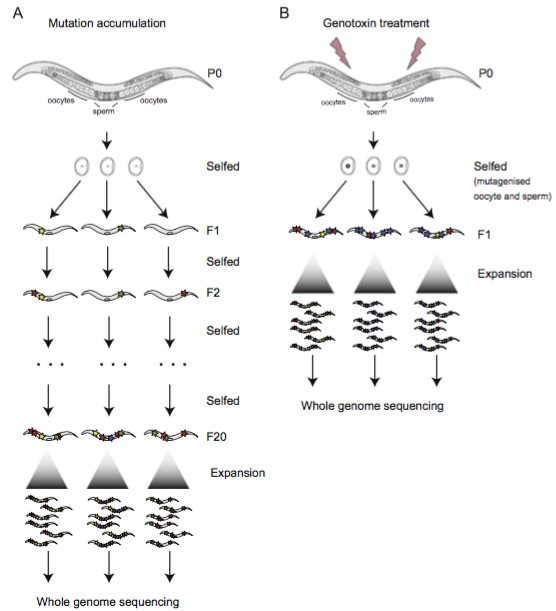
\includegraphics[scale=0.7]{two_exp_types.jpg}}
  \caption{Scheme of two worm experiment types. From Meier et al. 2014 \cite{Meier2}}
  \label{exp_types}
\end{figure}

Panel of cytotoxins consists of substances and exposures employed in cancer treatments: alkylating agents aflatoxin, cisplatin, dimethyl sulfate (DMS), ethyl methanesulfonate (EMS), methyl methanesulfonate (MMS), mechlorethamine (Mech) and hydroxyurea (HU), ionizing gamma-irradiation and X-rays.
List of genetic knock-outs includes genes representing all crucial DNA repair pathways: we consider 6 genes responsible for translesion synthesis, 13 backgrounds associated with single-strand break repair deficiency, 28 conditions associated with double-strand breaks repair deficiency, 6 helicases with different additional properties, 7 DNA damage checkpoint genes and 5 genes related to damage-caused cell death.
Full list of genetic conditions with respective pathways and their effects on genomic stability can be find in the Appendix.


\subsubsection*{Variant calling}

NGS data obtained from the experimental samples with Illumina sequencing at WTSI was further analyzed to extract genomic variants. Variant calling was performed separately for single nucleotide variants, small indels and large structural variants. The results have undergone a thorough filtering procedure to exclude technical errors, sequencing artifacts, caller mistakes and germline variance.

Individual SNVs were obtained using CaVEMan (\cite{caveman}) and separated from SNPs. Filtering for substitutions includes:
\begin{itemize}
\itemsep0em
\item uniqueness of each mutation (reported in only one sample)
\item artifacts removal: maximal coverage at the locus under consideration is 150 reads in control sample
\item no reads reporting variant in control sample
\item at least 20 percent of reads in test sample report variant
\item minimal coverage at the locus under consideration is 15 reads for both test and control samples
\item PCR errors identification: at least 1 read reporting variant in both directions
\item indel caused artifacts removal: no more than one read mapped with an indel across the base
\end{itemize}
After filtering, SNVs for every sample were classified into seven classes including dinucleotide substitutions as a separate class.

Indels (later classified into deletions, insertions and deletion-insertions) were called using Pindel (\cite{pindel}) and filtered according to the following criteria:
\begin{itemize}
\itemsep0em
\item uniqueness of each variant (reported in only one sample)
\item artifacts removal: maximal coverage at the locus under consideration is 150 reads in control sample
\item no reads reporting variant in control sample (up to 1)
\item PCR errors identification: at least 1 read reporting variant in both directions
\item no more than 8 repeat units at site
\item no sample in a panel of 5 control worms has variant in more than one read
\item at least 5 reads reporting variant
\end{itemize}

Structural variants were called using WTSI in-house software BRASS (\cite{NZ}), which extracts breakpoints via assembly from paired-end reads mapping. Filtering for the caller output includes quality control in the form of lower threshold for the number of reads reporting the variant, and repetitive events removal by filtering out all the variants reported at least once in the set of reference samples and deleting the intersecting events of the same type between all the samples.

Structural variants were reported in the form of pairs of breakpoints, which were further classified into the following categories:
\begin{itemize}
\itemsep0em
\item[$\square$] Tandem duplications
\item[$\square$] Deletions
\item[$\square$] Inversions
\item[$\square$] Complex events (more than 2 breakpoints classified as one event)
\item[$\square$] Intrachromosomal translocations
\item[$\square$] Interchromosomal translocations
\item[$\square$] Foldbacks (when one inversion-like breakpoint is present, i.e. polymerase is turning around and reversing the DNA without turning back again)
\end{itemize}

The final distribution of variants among different classes after the filtering procedures is shown in Figure N.

%\begin{figure}[h]
%  \centerline{\includegraphics[scale=0.5]{mut_classes.png}}
%  \caption{Overall distribution of mutations across all samples. Classes from "C$>$A" to "T$>$G" represent substitution classes, "NN$>$NN" - dinucleotide substitutions, "D" - small deletions, "I" - small insertions, "DI" - small deletion-insertions, "TD" - tandem duplications, "DEL" - large deletions, "INV" - invertions, "TRSL" - intrachromosomal translocations.}
%  \label{mut_distr}
%\end{figure}



\subsubsection{Homozygous and heterozygous mutations across generations}







\subsubsection{Extraction of mutational patterns}


\subsubsection*{Assumptions}

\textbf{Overdispersion modeling}. The current data shows signs of significant overdispersion for most of the response classes: residual deviance (i.e. the difference in likelihood for the model under consideration versus saturated) is significantly greater than the residual degree of freedom.



This is probably due to the limitations mentioned earlier: in some cases there was not enough time to see any mutations, which does not allow us to extract the corresponding factor contribution. The presence of overdispersion makes the current estimates of coefficient standard errors biased, which leads to incorrect assessment of coefficients significance and reduced prediction variance (\cite{overdisp}).

In order to account for an excess of zero results, we will turn to Gamma-Poisson model (also known as negative-binomial model), setting a Gamma prior on the coefficients as in \cite{Ivek} and \cite{BNB}, which will help to correctly estimate the actual variance of the result and make better predictions.

\textbf{Model quality assessment}. At the moment we estimate the confidence intervals for coefficients via bootstrapping to confirm stability of the estimates. The prediction error will be calculated by cross-validation procedure.

\textbf{Pattern identification}. We are going to perform unsupervised non-parametric clustering on the initial spectra utilizing hierarchical Dirichlet processes (\cite{Teh}), and try to map clusters to the signatures we extracted in order to confirm the ability to map the calculated effects back to the groups where they were applied.

\subsubsection*{Model}

To assess the individual contributions of every factor, we employed positive Poisson additive model with $r$ responses (reflecting the variant classes), that includes $k$ genetic, mutagenic, gene interaction and gene-mutagen interaction factors, for every response class $j$:

\[Y_{j} \sim Pois(\lambda_{j}), \lambda_{j} \in  \mathbb{R}_{+} , j = 1, ..., r\]

\begin{equation}
E[Y_j] = \lambda_j = X \beta_{j}^{T} = X_{gen} \beta_{j,gen}^T + X_{mut} \beta_{j,mut}^T + X_{int} \beta_{j,int}^T, \beta_j \in (\mathbb{R}_{+} \cup {0})^k
\end{equation}

To extract the model parameters, we further implemented non-negative matrix factorization with generalized Kullback-Leibler divergence minimization:

\[D(A||B) = \sum_{i,j} A_{ij} log(\frac{A_{ij}}{B_{ij}} ) - A_{ij} + B_{ij}\]

This approach is equivalent to maximum likelihood estimation in non-negative Poisson regression model in the case of fixed multiplier $X$: 

\[Y = X \beta, \beta \in M_{k \times r} (\mathbb{R}_{+} \cup {0})\]

\begin{equation}
\begin{split}
\ell(Y|X,\beta) &= \sum_{i,j} \left[Y_{ij}  log⁡(X \beta)_{ij} - (X \beta)_{ij} \right] + C \\
&= - \sum_{i,j} \left[Y_{ij}  log⁡ \left( \frac{Y_{ij}}{(X\beta)_{ij}} \right) - Y_{ij} + (X\beta)_{ij} \right] + \tilde{C} \\ 
&= - D(Y||X\beta) + \tilde{C}
\end{split}
\end{equation}

The update rule we used looks as follows:

\begin{equation}
\beta_{ij} \leftarrow \beta_{ij} \cdot \frac{\sum_s \frac{X_{si} Y_{sj}}{(X\beta)_{sj}}} {\sum_t X_{ti}}
\end{equation}

Coefficient matrix $\beta$ was update on every step till both the change in KL generalized distance \(D(Y||X\beta)\) and average change in the elements of $\beta$ reach the certain threshold. 

The variance and significance of the parameters calculated via NMF were estimated using Poisson maximum likelihood estimation and constrained Wald test (\cite{Wald}).


\subsubsection*{Benchmarking}



\subsubsection*{Method comparison}




%%%%%%%%%%%%%%%%%%%%%%%%%%%%%%%%%%%%%%%%%%%%%%%%%%


\subsection{Patterns of mutation accumulation under genotoxin exposure and DNA repair deficiency}


\subsubsection{DNA repair in \textit{C. elegans} and \textit{H. sapiens}}

\subsubsection*{Differences and similarities}

Signatures extracted for different genetic conditions also mostly coincide with the expected effects based on the function of the genes (\cite{p53}, \cite{Meier1},\cite{DNArepair}, \cite{DNAdamagerepair}). In the examples in the Figure N the following effects are presented: impact of ageing, \textit{brc-1} - BRCA1 ortholog encoding gene which contributes to homologous recombination, \textit{cep-1} - P53-like protein encoding gene which regulated damage-caused cell apoptosis, and \textit{smg-1} - kinase-related protein kinase SMG1 which regulates oxidative stress response.

\subsubsection*{Mutational signatures in mutations per generation}

\textit{rev-1} gene encodes an ortholog of human translesion polymerase REV1 which helps polymerases epsilon and delta to overcome stalled replication fork by inserting cytosins at abasic sites. As shown in Figure N, knocking out this gene does not significantly affect the mutational spectra in mutation accumulation experiment, but remarkably expands the mutational effects of DMS, which normally produces base substitutions and frameshift mutations and deletions.

\textit{xpa-1} encodes an ortholog of the human zinc finger protein XPA involved in nucleotide excision repair, which does not produce mutations when knocked-out alone, but expands the substitution mutational effects of alkylating agents and Gamma-irradiation, as shown in Figure N.





\subsubsection{Genetic interactions}

Apart from quantifying per-generation mutation rates for various knock-outs and effects of mutagen exposure, we have also identified several significant interaction effects, the underlying biology of which needs further investigation.

One example of a significant interaction between genetic backgrounds is the epistatic effect observed between mismatch repair system components \textit{pms-2} and \textit{pole-4}. \textit{pms-2} is a component of mismatch repair complex formed by attachment to \textit{mlh-1}. Both of these genes produce similar remarkable effects spectra when knocked-out, which agrees with the underlying biology (\cite{Denver}).

\textit{pole-4} is a catalytic subunit 4 of the ortholog of human polymerase epsilon, which is assumed to have mostly repair function correcting the errors made by polymerase delta. When knocked out on its own, this gene does not cause significant changes in the samples, but the double mutants with both defective \textit{pms-2} and defective \textit{pole-4} show a 3-fold increase in the overall mutation amount. Deficiencies in human polymerase epsilon and polymerase delta were previously reported as driver genes in hypermutated brain cancers (\cite{Shlien}).





\subsubsection{Mutagen exposures}

Using this approach, we calculated the qualitative effect estimations for all of the factors. Effects for genotoxins used in the study are consistent with their chemical interactions with DNA known from literature (\cite{Helleday}, \cite{DNAdamagerepair}, \cite{Meier1}) and can be found in Figure N.





\subsubsection{Relation to various genomic features}

\subsubsection*{Transcription}

\subsubsection*{Replication directionality}

\subsubsection*{Localisation of mutations}

Microhomology, telomeres, clusters

\subsubsection*{Epigenetic features}

\textbf{Incorporation of additional genetic information}. This includes validation of structural variants (namely, deletions and duplications) by analyzing copy number changes in the sample genomes, GC-content adjustment for correct comparison of substitutions types proportions, and removal of variants coming from low-complexity regions and highly repetitive regions. 

\subsubsection*{Mitochondrial DNA}

%%%%%%%%%%%%%%%%%%%%%%%%%%%%%%%%%%%%%%%

\subsection{Translation of mutational signatures between model organisms and human cancers}

\subsubsection{Mutational patterns of mismatch repair}

\subsubsection{Other DNA repair pathways}

\subsubsection{Differences and similarities in response to mutagen exposure}

Relevance to cancer

DNA repair pathways

Mutagens, cancers related to environmental exposure



%%%%%%%%%%%%%%%%%%%%%%%%%%%%%%%%%%%%%%%

\subsection{Limitations of the analysis}


The current model concept does not account for several limitations coming from the nature of the data:
\begin{itemize}
\itemsep0em
\item Restricted number of mutations - some rearrangement can not be produces in sufficient number (negative selection)
\item Small number of replicates for each experiment (makes it hard to estimate the variance of the results)
\item Negative selection: some rearrangements can not be reproduces in sufficient number (amount of junk DNA is extremely low)
\end{itemize}

To make the model as useful as possible, at the moment we are working on the following aspects:

\subsection{Discussion}




%\newpage{}

%\appendix
%\section*{Appendix. Table of genetic knock-outs and mutagens used in the study with their interactions.}

%\begin{table}[h!]
%\centering
%\begin{adjustbox}{width=1\textwidth}
%\begin{tabular}{1.0*\textwidth}{|c|c|c|c|c|c|c|c|c|c|c|c|}
%\hline 
% & None & Aflatoxin & Cisplatin & DMS & EMS & HU & Mec & MMS & Rad & Xray & Pathway\tabularnewline
%\hline \hline
%N2 & allsubs, D, I, allSVs - INV  &  C$>$A & C$>$A, D & T$>$C, T$>$A, C$>$T, TD & allsubs, D  & C$>$T, C$>$A & D & allsubs – C$>$G, D, TD & allsubs, D & C$>$T, C$>$A, D, TD, INTCHR & \tabularnewline
%\hline 
%agt-1 & TD & & & & C$>$T, T$>$A & T$>$C, T$>$A, C$>$T &  &  &  &  & translesion synthesis	\tabularnewline
%\hline 
%\end{tabular}
%\label{app_table}
%\end{adjustbox}
%\end{table}

\end{document}

\newpage{}


\begin{document}

\pagestyle{empty}

\chapter{Interactions between DNA damage and repair}

\section{Introduction}

Mutational signatures result from the DNA repair activity on the lesions caused by mutagenic
processes; however, previously these signatures were always assumed to be consistent across different 
sources of mutation data. Given the double-sided nature of mutation acquisition, it seems 
reasonable to assume that changes in the DNA repair component availability
may affect the mutational signatures of exogenous or endogenous mutagenic agents.

In this chapter, I will introduce the means for quantifying the contribution of different factors and their
interactions to the mutational spectra of samples with combined DNA repair deficiency and mutagen
exposure. By studying the most striking examples and presenting a summary of interaction effects,
I will show that the interplay between DNA repair and damage is common, can alter the signature
of the mutagen, or make it look like the signature of another mutagen due to the switch of DNA repair
pathway to process the damage. This chapter will also further stress the fact that the strongest
mutational signals -- the ones which are first to be picked up by various factor analysis methods
-- usually result from non-linear interaction of different factors, not a simple combination of
the underlying components.

%%%%%%%%%%%%%%%%%%%%%%%%%%%%%%%%%%%%%%%%%%

\section{DNA repair status as a proxy to treatment sensitivity}

***Talk about interaction data from other sources***

\begin{figure}[h]
  \centering
\centerline{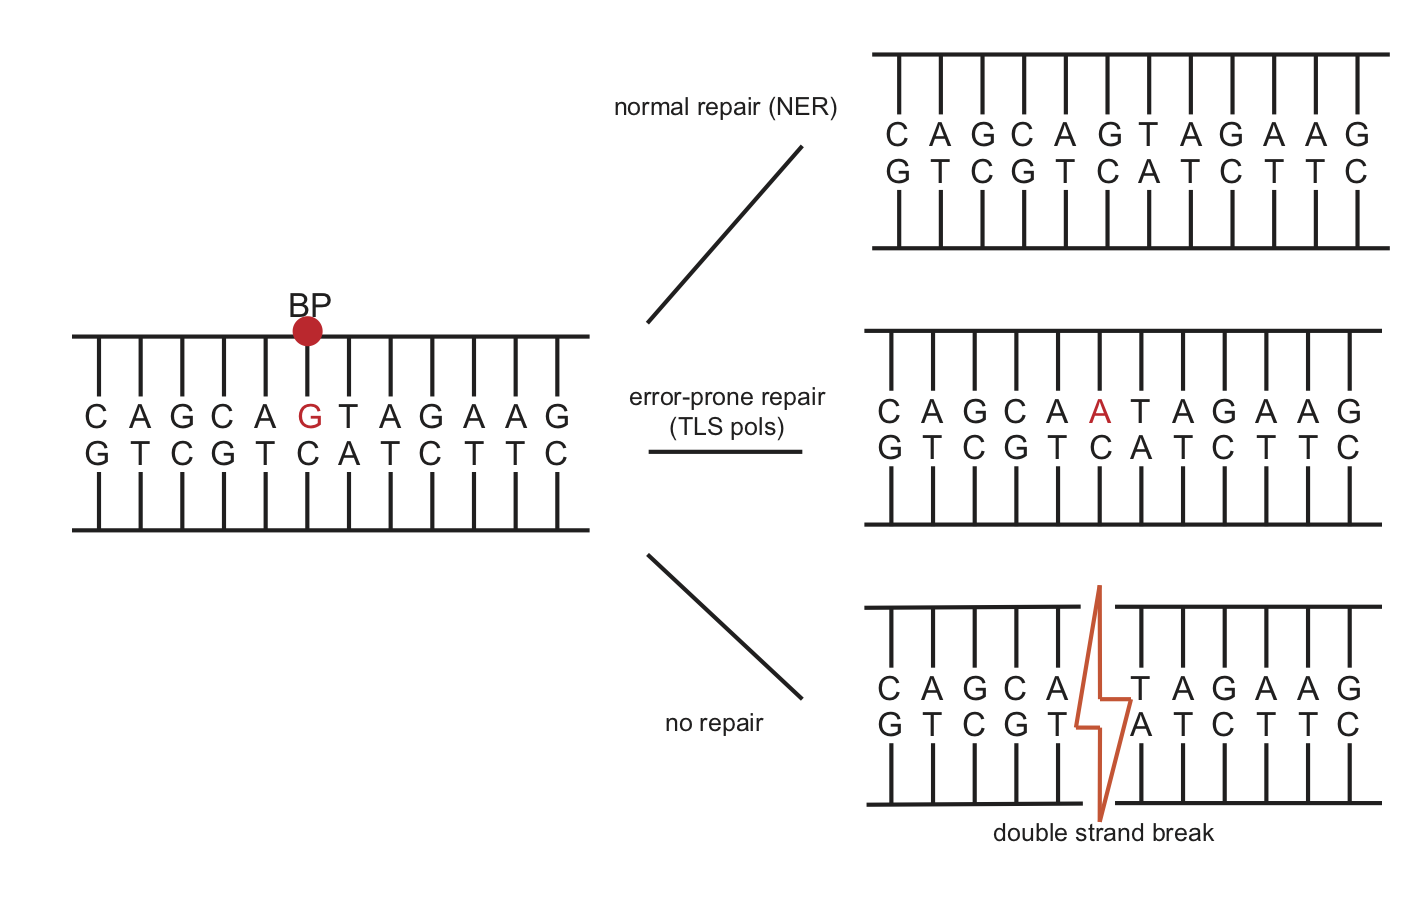
\includegraphics[width=1\textwidth]{figures/interaction_concept.png}}
  \caption{The precise type of mutation observed depends on the repair available. BP - Benzo-[a]-pyrene adduct.}
  \label{interaction_concept}
\end{figure}

\section{Quantifying interaction effects in a controlled experimental model}

The controlled nature of the mutagenesis screen allowed us to take a step further into dissection 
of contributions of DNA repair and DNA damage to the mutational spectra of \textit{C. elegans} samples.

Having the full information on the relative amount of exposure to each signature for each sample, it was possible to go beyond the recognition of the repetitive patterns and quantify the actual amount of change introduced by each interaction. Most of current mutagenesis models only account for non-negative effects: additional factors can only add mutations, but the data from certain experiments indicated that mutagenesis can in fact be reduced ***ref a figure from Chapter 2 here***. Hence the model should be able to reflect both amplification or reduction of existing signatures as well as transformation of genotoxin induced signatures.

In order to fulfill this task while maintaining interpretability of all model components, we developed a hierarchical Bayesian model which adapts all of the possible changes and noise sources in the data. 

\subsection{Bayesian modelling}

***TODO: why we used a hierarchical bayesian model***

For each of the mutation types $i$ and
samples $j$ we counted the respective number of mutations per sample $Y_{j,i}$.

As a first step, we use the mutation accumulation data to define a prior on signatures of DNA repair deficiencies, so that we could leverage the information from all mutant samples towards the refinement of signatures of genetic backgrounds. The posterior distribution will then be calculated using the rest of the samples. In the first stage, for each of the mutation accumulation samples, the mutation counts $Y \in \mathbb{R}_{+}^{119}$ were modeled by a negative binomial distribution,
\[Y \sim NB( \mu, \phi=100), \]
with expectation
\[ \mu = g \cdot G^{*} \cdot S_{G}^{*}.\]

Here $g$ denotes the adjusted generations in the absence of a mutagenic exposure as in Chapter 2. $G^{*}$ is a binary indicator matrix of genotypes, and $S_{G^{*}} \in Mat_{119\times51}(\mathbb{R}_{+})$ is a matrix of signatures of mutation accumulation effects per genotype (star denotes the subset of data where mutation accumulation data is available).

We used a log-normal prior distribution for these signatures, $S_{G^{*}} \sim logN(0, \sigma^{2}_{G})$ iid with a scalar variance $\sigma^{2}_{G}$. In total, we used 451 samples from mutation accumulation experiments with generation number higher than 1, and obtained signatures for 51 genotypes (\textit{agt-1}, \textit{exo-1}, \textit{rad-51} knockouts did not have mutation accumulation experiments).

In the next stage, the mutation counts for a given sample
$Y_{N,1:119}$ were modeled by a negative binomial distribution,

\[Y \sim \mathbb{NB} (\mu, \phi = 100), \]

with expectation
\[\mu = \mu_{G} \cdot (g + \alpha_{I}) + d \cdot \mu_{M} \cdot \beta_{I},\]

Here $\mu_{G} = G \times S_{G}^{T} \in \mathbb{R}_{2721\times119}^{+}$ describes 
the mutations expected due to the genetic background, with $G$ denoting an 
indicator matrix of genotypes per sample and $S_{G}$ being a matrix of 
mutational signatures of the genetic knockouts with a prior $S_{G} \sim \Gamma(shape_{G}, rate_{G})$ 
fitted to the posterior draws for $S_{G^{*}}$. 
Similarly, $\mu_{M} = M \cdot S_{M} \in \mathbb{R}^{+}_{2721 \times 119}$
is the expectation for the mutations created by mutagen M at median dose, 
with $M \in {0,1}^{2721 \times 12}$ being the indicator for the 12 mutagens 
used in this screen, and $S_{M} \in \mathbb{R}_{+}^{12\times119}$ being their 
signatures in wildtype, with per-column prior $S_{M}^{(j)} \sim logN\left(0, \sigma_{Mj}^2\right)$, where the variances $\sigma_{M}^2 = \left(\sigma_{M1}^2, ..., \sigma_{M12}^2\right)$ have prior distributions $\sigma_{Mj}^2 \sim \Gamma(1,1)$ iid. 
The terms $\alpha_{I} \in \mathbb{R}_{+}^{2721}$ and $\beta_{I} \in \mathbb{ℝ}_{+}^{196 \times 119}$ model how these terms interact. The scalar 
term for the genotype is linear with respect to the mutagen dose,

\[\alpha_{I} = d \cdot (I \cdot b_{I}) + (J \cdot a_{J}),\]

with $I \in {0,1}^{22721 \times 196}$ and $J \in {0,1}^{2721 × 208}$ being binary 
indicator matrices for all interactions and all mutagenesis experiments 
(i.e. interactions and wild-type mutagenesis experiments), respectively. 
Rates $b_{I} \in \mathbb{R}_{+}^{196}$  and offsets $a_{I} \in \mathbb{R}_{+}^{208}$ 
were modelled as log-normal distributed random variables,
$a_{I} \sim logN(0,0.5)$ and $b_{I} \sim logN(0,0.5)$. 
The rationale behind this parameterisation is that the \textit{C. elegans} 
strain used for the experiment may have slightly diverged, 
thereby adding $a_{I} \cdot S_{G}$ mutations with the same spectrum 
as in the absence of a mutagen. In addition to that, mutagen 
exposure can amplify the mutation types specific to the genotype, 
as in case of alkylating agent treatment of \textit{rev-3} deficient samples, 
and hence the mutagen exposure of dose d may add $d \cdot b_{I}$ mutations 
of the mutagen-free spectrum.

The main assumption about interaction effects is that the wild-type spectrum 
of the mutagen $S_M$ may change by the factors $\beta_{I} \in \mathbb{ℝ}_{+}^{119 \times 196}$ measuring the fold-change of each mutation type which is expressed as 

\[\beta_{I} = I \times S_{I},\] 

where $S_{I} \in \mathbb{R}_{+}^{196 \times 119}$ is the fold-change 
with 119 terms per interaction, with a prior distribution 
$log(S_I^{(j)}) \sim Laplace(0, \sigma_{Ij}^{2})$, all $\sigma_{Ij}^{2} \sim \Gamma(1,1)$ iid.

\subsection{Parameter estimation using Hamiltonian Monte-Carlo}

***TODO: about the HMC and convergence***

The overdispersion parameter $phi=100$ was selected based on the estimates of overdispersion in the dataset when fitting a negative binomial distribution with a shared overdispersion parameter to all the experiments in the dataset. It allows to account for additional variation within the replicates as well as for overflow of zeros which could present a problem in a Poisson framework.

The model was specified using R-package "greta" (Golding 2018), and the posteriors of $S_{G}$, $S_{M}$, $S_{I}$, $a_{J}$, $b_{I}$ and hyperparameters $\sigma^{2}_{M}$, $\sigma_{I}^{2}$ were estimated using Hamiltonian Monte Carlo sampling. We used 2000 steps for warmup and 5000 steps over 4 chains to ensure the best possible convergence. The point estimates for the parameters were taken as means of the samples across all chains. The relevant R codes are published on Github under \url{github.com/gerstung-lab/signature-interactions}.

EMS exposure was the only genotoxin for which we observed very different mutation counts across different experiments in wildtype. Respective samples were coming from 5 batches, which are stated in the ‘Comments’ section of the samples description table in Supplementary Table 1. In order to account for this effect, we introduced additional factor ={i}, i=1,...,4 which accounted for the log-difference in real dose applied to the samples in batches 2 to 5 compared to batch 1 which was considered as reference. The prior distribution for these adjustment was taken as iN(0,0.5)iid.  The dose for these samples was then calculated as d' = d*ebatch*, where batch{0,1}27214 is a binary matrix reflecting if a sample belongs to any of the batches 2-5. These adjustments were estimated along with the rest of the coefficients.

Combined genotype-mutagen interactions were tested for effect in two settings: altering the total number of base substitutions, and changing the distribution of mutations. The fold-change in the number of single base substitutions was calculated as predicted with interactions versus the one predicted without interactions using 2000 out of 10000 samples draws across 4 chains for all 196 interactions. The change in profile was quantified by calculating the cosine distance between the expected profiles with and without interactions, and those with distance higher than 0.2 were considered different. As all of the interactions which showed a change in signature appearance also came up in burden analysis, we only applied hypothesis testing (chi-square test for log(E(FCs))for s = 1, … 196) and Benjamini-Hochberg FDR control procedure for the set of substitution burden fold-changes.

%%%%%%%%%%

\section{Alteration of mutagen profiles in \textit{C. elegans} experiments}

\subsection{Alkylating agents and corresponding repair enzymes}

Among all of the interaction experiments, the higher number of mutations was observed for the knockout of TLS polymerase \textit{polk-1} under exposure to alkylating agents MMS and DMS. Absence of POLK-1 led to a 40x increased mutation rate per unit of genotoxin (1 mM for MMS, and 0.1 $\mu$M for DMS) as well as a visible change in the spectrum of mutations (Figure \ref{polk1mms}). T$>$A transversions increased $\sim 30$x, expecially in TpTpC and TpTpT contexts, and other mutation types including SNVs and MNVs were 10 times elevated. 

\begin{figure}[h]
  \centering
\centerline{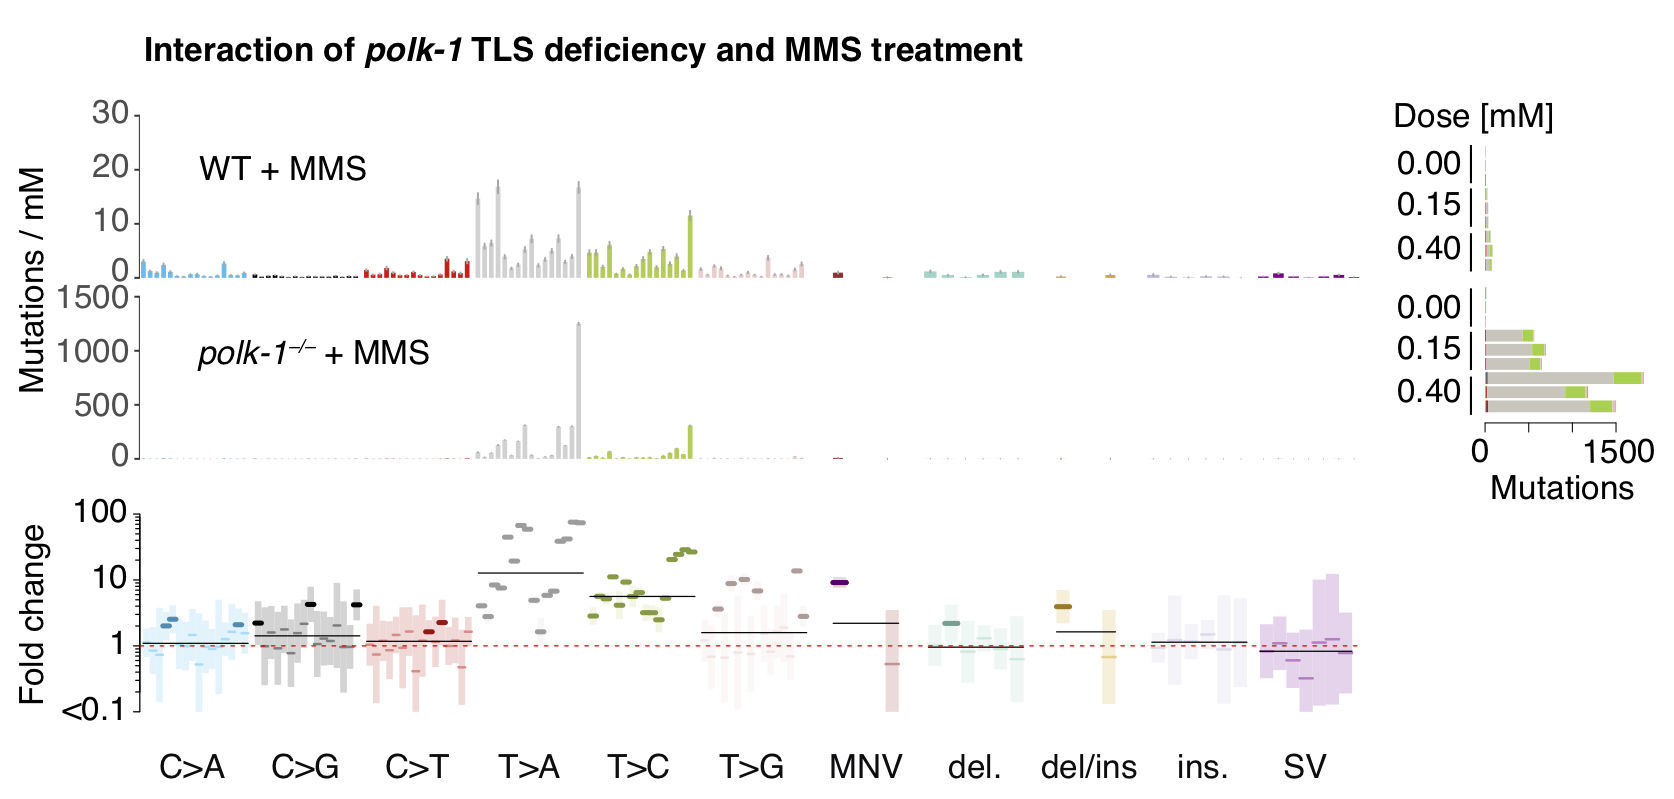
\includegraphics[width=1\textwidth]{figures/polk-1-MMS-interaction.png}}
  \caption{Mutations introduced per unit of MMS in wild-type (top panel) and in \textit{polk-1} deficient mutants (central panel), along with the fold-change per mutation type (bottom) and total numbers of mutation in response to different doses of mutagen (right panel).}
  \label{polk1mms}
\end{figure}


A similar change of the mutation spectrum was observed for DNA ethylation by EMS, however at a reduced rate of about 10x. This change in mutation spectrum reveal diverging repair of alkylated guanines and adenines: N3-methyladenosine, unlike O6-methylguanine, stalls replicative polymerases, which is overcome by TLS polymerase POLK-1, usually at the expense of fidelity, often incorporating false nucleotides9. Our data indicate that bypass by POLK-1 in wild type worms is relatively error free leading to the correct incorporation of a thymine on the opposing strand in most cases. Yet in the polk-1 mutant, bypass has to be achieved by other TLS polymerases, which results in increased T>N mutagenesis particularly favoring incorporation of an adenine leading to predominant of T$>$A mutations. 

Conversely, O6-methylguanine, another modification inflicted by the methylating agents MMS and DMS, leads to G:T mispairing resulting in C$>$T transitions and is repaired by distinct repair pathways. Knockout of the alkyl-transferase \textit{agt-1} increases C>T mutations by a factor of 4 under methylating MMS exposure, demonstrating that \textit{agt-1} removes most O6-methyl-guanine adducts error-free, thus acting as the functional C.elegans ortholog of the human methyl guanine methyl transferase MGMT. Interestingly, one observes a similar, but weaker interaction of \textit{agt-1} with the ethylation agent EMS, leading to an increase C>T transitions by a factor of 1.5, indicating that \textit{agt-1} is involved in, but less efficient at, removing ethyl groups. A knockout of the second alkyltransferase present in C. elegans, \textit{agt-2}, showed even smaller effect on O6-eG repair (increase by 20\% per average dose). Moreover, we also observe a uniformly increased MMS and DMS mutagenesis under knockouts of base excision repair (apn-1) and nucleotide excision repair (\textit{xpa-1}, \textit{xpf-1}; 1.2x and 2x, respectively), as well as a 1.2x increase of C$>$T mutations in mismatch repair knockout of \textit{mlh-1}, indicating that O6-meG:C pairs may be recognised and repaired by the components of these systems.

\subsection{Translesion synthesis and various mutagens}

Knockout of two other translesion polymerases, POLH-1 and REV-3, without exogeneous genotoxicity leads to a mutation pattern characterised by deletions in the range of 50-400 bp, thought to arise via the formation of DNA double strand breaks and \textit{polq-1} mediated repair. To protect the genome from such deleterious mutations, it is believed that TLS bypass such lesions at the cost of a higher base substitution rate. In line with this notion, we observed a 3-fold reduction in substitutions and 10-fold increase in indels in \textit{rev-3} knockouts under exposure with UV, and a 2-fold decrease in substitutions in \textit{polh-1} mutants under EMS exposure, indicating that DNA repair in some cases adds to overall mutagenicity.

\subsection{Nucleotide excision repair deficiency exaggerates the effects of mutagens}

In contrast to the the above examples where repair deficiency leads to both increase in mutagenesis but also to alteration of mutational spectra, the knockouts of the NER genes \textit{xpf-1} and \textit{xpc-1} increased the rate of UV-B induced mutagenesis by factors of 10 and 35, respectively. The fold-change appears to be relatively uniform across the entire mutation spectrum, indicating that NER is involved in repairing the large majority of UV-B damage of different types, including both single- and multinucleotide lesions (Fig. 3g). Interestingly, \textit{xpf-1} knockout also uniformly increased the mutation burden due to alkylation by a factor of 2 indicating that alkylation damage is eventually repaired by NER. Similarly \textit{xpf-1} knockouts also showed an two-fold increase in mutations after aristolochic acid, demonstrating that NER repairs both small and bulky adducts.


\subsection{Widespread interaction effects across the screen and mutation summary}

These examples of genotoxin-repair interactions are not uncommon: In total, 72/196 (37\%, at FDR of 10\%) of combinations displayed an interaction between DNA repair status and genotoxin treatment. Conversely, more than half of combinations produced mutation spectra which could be fully described as the superposition of the wild-type genotoxin signature and that of the DNA repair deficiency background, indicating that the two processes acted independently. Usually genotoxin-repair interactions increase the numbers of mutations obtained for a given dose of mutagen, leaving the mutational spectrum mostly unchanged, others have a profound impact on mutational spectra (Figure 4B, for a comprehensive list of effects see Supplementary Figure 5 and Supplementary Table 3). The emergence of distinct mutational spectra depending on DNA repair status reflects how multiple repair enzymes and pathways contribute to mending damaged DNA as in the case of DNA alkylation. If DNA repair is predominantly achieved by one pathway such as by NER for UVB damage and bulky DNA adducts, the number of mutations is increased, but the signature tends to remain unchanged.

To illustrate the overall magnitude of these interaction effects, we estimate that of the 141,004 mutations we observed upon treatment with genotoxins in DNA repair deficient strains 23\% of mutations were attributed to the endogenous mutagenicity of DNA repair deficiency genotypes independent of genotoxic exposure, and 62\% of mutations would be attributed to genotoxic exposures independent of the genetic background. Of these, 2\% were not observed due to negative interactions of genotoxins and DNA repair deficiency, such as UVB exposure of TLS knockout strains, and 17\% of mutations were added because of the positive interactions, which increased mutagenicity.

In summary, the above examples and analysis demonstrate that the combination of DNA damage and DNA repair deficiency can yield mutational patterns which can not be explained by the mere superposition of patterns resulting from exposure of wild-type DNA repair proficient strains and mutagenesis induced in repair defective strains in the absence of external mutagenesis. The alteration of mutational pattern by DNA repair status appears most remarkable when multiple repair enzymes and pathways contribute to mend damaged DNA as in the case of DNA alkylation. If repair is predominantly affected by one pathway such as NER for UV damage and bulky DNA adducts, the number of mutations is increased but the spectrum tends to remain unchanged.

\subsubsection*{Evidence of interactions from other sources}

Data from other model experiments???

Metabolic activation of mutagens in mammals???


%%%%%%%%%%%%%%%%%%%%%%%%%%%%%%%%%%%%%%%%%%

\section{Discussion}

In this chapter, I presented a way of quantifying the degree of interaction between
genetic and mutagenic factors in controlled experiments on \textit{C. elegans}, and performed
a comparison of effects across 196 combinations of repair components and damaging agents
which showed the diversity and abundance of significant interaction effects which may
be both positive and negative. I also demonstrated how these interactions may increase
or decrease the total burden, and they may alter the signature of the mutagenic agent
as well as intensify the signature of genetic factors.

This analysis shows that the signatures of many mutagenic processes are not necessarily
consistent: depending on the DNA repair availability, their contributions will be different
and not aligned with the exposure dose, and their mutational spectra can change partially or
completely. It opens the way for considering DNA repair status as a factor in signature
decomposition as it may alter the appearance of latent components or introduce additional ones.

Studying the effects of DNA repair deficiencies on the mutagenic exposures also provides
insights into the mechanisms of repair and specificity of the damage. The screen above only
considers mutations, i.e. results of repair-damage interplay; combined with the analysis
of unrepaired damage, which may be detected with direct damage detection methods including
Nanopore sequencing and other techniques, it could provide a comprehensive and quantitative
picture of mechanisms of damage and repair of the genomic DNA.

Another limitations which needs to be taken into account is the simplicity of mutagen intake
in \textit{C. elegans} which does not necessarily correspond to the processing applied upon 
mutagenic agents in human body, as was mentioned in the Chapter 1. Metabolic activation, 
differences in sensitivity or repair across tissues, or other ways of substance 
processing may completely alter mutagenic activity of certain agents or of the repair activity,
hence a further investigation of these effects in human cells and organs deems necessary.

In the next chapter, I will explore the range of repair-damage interaction in human
cancers by modifying the signature extraction model and incorporating additional information
about DNA repair status of the samples.

\end{document}







\newpage{}



\begin{document}
\pagestyle{empty}
\section{Implications for cancer signature analysis}

Motivation: uncertainty in signature assignment and definition


\subsection{Methods and resources}

\subsubsection{Data sources and acquisition}

Individual studies, TCGA, ICGC, PCAWG

Filtering and QC

\subsubsection{Analysing DNA repair efficacy}

Sample labeling: search for signs of defective repair components

\subsubsection{Methods for extraction of signature alterations}

\subsubsection*{MCMC for effect extraction}

\subsubsection*{Expanded model for simultaneous exposure, signature and effect extraction}


%%%%%%%%%%%%%%%%%%%%%%%%%%%%%%%%%%%%%%%

\subsection{Analysis of publicly available data}

\subsubsection{Clinically targetable interactions}

Interactions as a source of therapy targets: temozolomide and MGMT, BRCA and PARP inhibitors, APOBEC and ATR inhibitors

\subsubsection{Significance of DNA repair genes}


\subsubsection{Interactions of DNA repair and damage factors detectable in human cancers}

Interactions observed in human data

Illustration:

\subsubsection*{temozolomide}

\subsubsection*{APOBEC and BER}

\subsubsection*{POLE-MMR}

\subsubsection*{NER/FA and cisplatin}

Prospective interactions which are not represented in the data yet

Signature 17 may be a result of mutagenic activity and interact with NER status

Other environmental agents (asbestos, alcohol?)

%%%%%%%%%%%%%%%%%%%%%%%%%%%%%%%%%%%%%%%

\subsection{Discussion}

\subsubsection*{what we expected but never detected}

\end{document}

\newpage{}


\begin{document}
\pagestyle{empty}
\section{Conclusions}

\subsection*{What is done}

Variability of mutational profiles across different DNA repair mutations

Prevalence of interaction effects between DNA repair components and damaging agents

Translation of studies in model organisms to human cancers

Limitations to signature analysis in cancers


\subsection*{What does it say}


\subsection*{What could also be done}


Significance for mutagenesis field: comprehensive catalogue of high-resolution profiles for a wide range of genetic knock-outs and mutagens

Significance for clinical research: bringing together whole-genome/exome profiling and targeted tests

Implications for diagnostics, treatment, resistance

Limitations: low signal in worm data, variance, high noise in human data, timing and clonality issues, technological limitations

Future work





\end{document}


\newpage{}


\begin{thebibliography}{1}

\bibitem{DNArepair} Alberts, B., Johnson, A., Lewis, J. et al. \textit{Molecular Biology of the Cell}. 4th edition. New York: Garland Science; 2002.

\bibitem{Alex1} Alexandrov, L.B. et al. 2013. Signatures of mutational processes in human cancer. \textit{Nature} \textbf{500}, 415-421.

\bibitem{Alex2} Alexandrov, L.B., Nik-Zainal, S., Wedge, D.C., Campbell, P.J. and Stratton, M.R. 2013. Deciphering signatures of mutational processes operative in human cancer. \textit{Cell Rep.} \textbf{3}, 246-259.

\bibitem{Alex3} Alexandrov, L.B., Jones, P.H., Wedge, D.C., Sale, J.E., Campbell, P.J., Nik-Zainal, S. and Stratton, M.R. 2015. Clock-like mutational processes in human somatic cells. \textit{Nature Genetics} \textbf{47}, 12, 1402-1407.

\bibitem{Alex4} Alexandrov, L.B. and Stratton, M.R. 2014. Mutational signatures: the patterns of somatic mutations hidden in cancer genomes. \textit{Curr. Opin. Genet. Dev.} \textbf{24}, 52-60.

\bibitem{Alex5} Alexandrov, L.B., Nik-Zainal, S., Siu, H.C., Suet, Y.L. and Stratton, M.R. 2015. A mutational signature in gastric cancer suggests therapeutic strategies. \textit{Nature Communications} \textbf{6}, 8683.

\bibitem{Cemgil} Cemgil, A.T. 2009. Bayesian Inference for Nonnegative Matrix Factorisation Models. \textit{Computational Intelligence and Neuroscience} 2009.

\bibitem{Denver} Denver, D.R., Feinberg, S., Estes, S., Thomas, W.K. and Lynch, M. 2005. Mutation Rates, Spectra and Hotspots in Mismatch Repair-Deficient Caenorhabditis Elegans. \textit{Genetics} \textbf{170}, 107-113.

\bibitem{Flibotte}  Flibotte, S. et al. 2010. Whole-genome profiling of mutagenesis in Caenorhabditis elegans. \textit{Genetics} \textbf{185}, 431-441.

\bibitem{COSMIC} Forbes, S.A. et al. 2014. COSMIC: exploring the world's knowledge of somatic mutations in human cancer. \textit{Nucl. Acids Res.} \textbf{43}, 805-811.

\bibitem{DNAdamagerepair} Friedberg, E.C., Walker, G.C. and Siede, W. \textit{DNA repair and mutagenesis}. Washington, D.C.: ASM Press; 1995.

\bibitem{Helleday} Helleday, T. et al. 2014. Mechanisms underlying mutational signatures in human cancers. \textit{Nat. Rev. Genet.} \textbf{15}, 585-598.

\bibitem{overdisp} Hinde, J. and Demetrio, C.G.B. 1998. Overdispersion: Models and estimation. \textit{Computational Statistics and Data Analysis} \textbf{27}, 151-170.

\bibitem{Hollstein} Hollstein, M., Alexandrov, L.B., Wild, C.P., Ardin, M. and Zavadil, J. 2016. Base changes in tumour DNA have the power to reveal the causes and evolution of cancer. \textit{Oncogene} (2016), 1-10.

\bibitem{Ivek} Ivek, I. 2014. Probabilistic Formulations of Nonnegative Matrix Factorization. \textit{Computer Science Seminars at Ruder Boskovic Institute}.

\bibitem{Lee} Lee, D.D., Seung, H.S. 2000 Algorithms for non-negative matrix factorization. In \textit{Advances in Neural Information Processing} \textbf{13} (Proc. NIPS*2000).

\bibitem{Meier1} Meier, B., Cooke, S.L., Weiss, J., Bailly, A.P., Alexandrov, L.B., Marshall, J., Raine, K., Maddison, M., Anderson, E., Stratton, M.R., Gartner, A., Campbell, P.J. 2014. C. elegans whole-genome sequencing reveals mutational signatures related to carcinogens and DNA repair deficiency. \textit{Genome Research} \textbf{24}, 1624-1636.

\bibitem{Meier2} Meier, B., Gartner, A. 2014. Having a direct look: Analysis of DNA damage and repair mechanisms by next generation sequencing. \textit{Experimental Cell Research} \textbf{329}, 35-41.

\bibitem{Wald} Molenberghs, G., and Verbeke, G. 2007. Likelihood Ratio, Score, and Wald Tests in a Constrained Parameter Space. \textit{The American Statistician} \textbf{61}, 22-27.

\bibitem{NZ} Nik-Zainal, S. et al. 2012. Mutational processes molding the genomes of 21 breast cancers. \textit{Cell} \textbf{149}, 979-993.

\bibitem{NZ2} Nik-Zainal, S. et al. 2016. Landscape of somatic mutations in 560 breast cancer whole-genome sequences. \textit{Nature} \textbf{534}, 47-54.

\bibitem{Poon1} Poon, S.L. et al. 2014. Mutation signatures of carcinogen exposure: genome-wide detection and new opportunities for cancer prevention. \textit{Genome Med.} \textbf{6}, 24.

\bibitem{Poon2} Poon, S.L., Huang, M.N. et al. 2015. Mutation signatures implicate aristolochic acid in bladder cancer development. \textit{Genome Medicine} \textbf{7(1)}, 38. 

\bibitem{p53} Rivlin, N., Brosh, R., Oren, M. and Rotter, V. 2011. Mutations in the p53 Tumor Suppressor Gene. \textit{Genes Cancer.} \textbf{2(4)}, 466-474.

\bibitem{Roberts} Roberts, S.A. and Gordenin, D.A. 2014. Hypoermutation in human cancer genomes: footprints and mechanisms. \textit{Nature Reviews} \textbf{14}, 786-800.

\bibitem{Segovia} Segovia, R., Tam, A.S., and Stirling, P.C. 2015. Dissecting genetic and environmental mutation signatures with model organisms. \textit{Trends Genet.} \textbf{31(8)}, 465-474.

\bibitem{Shlien} Shlien, A., Campbell, B.B., de Borja, R., Alexandrov, L.B., Merico, D., Wedge, D. et al. 2014. Combined hereditary and somatic mutations of replication error repair genes result in rapid onset of ultra-hypermutated cancers. \textit{Nature Genetics} \textbf{47}, 257-262.

\bibitem{caveman} Stephens, P.J., Tarpey, P.S. et al. 2012. The landscape of cancer genes and mutational processes in breast cancer. \textit{Nature} \textbf{486}, 400-404.

\bibitem{Stratton} Stratton, M.R., Campbell, P.J. and Futreal, P.A. 2009. The cancer genome. \textit{Nature} \textbf{458}, 719-724.

\bibitem{MMR} Supek, F. and Lehner, B. 2015. Differential DNA mismatch repair underlies mutation rate variation across the human genome. \textit{Nature} \textbf{521}, 81-84.

\bibitem{Teh} Teh, Y.W., Jordan, M.I., Beal, M.J. and Blei, D.M. 2006. Hierarchical Dirichlet Processes. \textit{Journal of the American Statistical Association} \textbf{101(476)}, 1566-1581

\bibitem{Tian} Tian et al. 2015. Computational methods and resources for the interpretation of genomic variants in cancer. \textit{BMC Genomics} \textbf{16(8)}.

\bibitem{KRAS} Wang, M.T. et al. 2015. K-Ras Promotes Tumorigenicity through Suppression of Non-canonical Wnt Signaling. \textit{Cell} \textbf{163(5)}, 1237-51.

\bibitem{Wu} Wu, S., Powers, S., Zhu, W. and Hannun, Y.A. 2016. Substantial contribution of extrinsic risk factors to cancer development. \textit{Nature} \textbf{569}, 43-47.

\bibitem{pindel} Ye K., Schulz M.H., Long Q., Apweiler R., Ning Z. 2009. Pindel: a pattern growth approach to detect break points of large deletions and medium sized insertions from paired-end short reads. \textit{Bioinformatics} \textbf{25(21)}, 2865-71..

\bibitem{BNB} Zhou, M. et al. 2012. Beta-Negative Binomial Process and Poisson Factor Analysis. \textit{International Conference on Artificial Intelligence and Statistics} (AISTATS2012), JMLR W\&CP, \textbf{22}, 1462-1471.

\end{thebibliography}

\newpage{}

\end{document}
